\documentclass{beamer}

\mode<presentation> {
% Colors

% \usetheme{default}
% \usetheme{AnnArbor}
% \usetheme{Antibes}
% \usetheme{Bergen}
% \usetheme{Berkeley}
% \usetheme{Berlin}
% \usetheme{Boadilla}
% \usetheme{CambridgeUS}
% \usetheme{Copenhagen}
% \usetheme{Darmstadt}
% \usetheme{Dresden}
% \usetheme{Frankfurt}
% \usetheme{Goettingen}
\usetheme{Hannover}
% \usetheme{Ilmenau}
% \usetheme{JuanLesPins}
% \usetheme{Luebeck}
% \usetheme{Madrid}
% \usetheme{Malmoe}
% \usetheme{Marburg}
% \usetheme{Montpellier}
% \usetheme{PaloAlto}
% \usetheme{Pittsburgh}
% \usetheme{Rochester}
% \usetheme{Singapore}
% \usetheme{Szeged}
% \usetheme{Warsaw}

%Themes

% \usecolortheme{albatross}
% \usecolortheme{beaver}
% \usecolortheme{beetle}
% \usecolortheme{crane}
% \usecolortheme{dolphin}
% \usecolortheme{dove}
% \usecolortheme{fly}
% \usecolortheme{lily}
% \usecolortheme{orchid}
% \usecolortheme{rose}
% \usecolortheme{seagull}
\usecolortheme{seahorse}
% \usecolortheme{whale}
% \usecolortheme{wolverine}

%\setbeamertemplate{footline} % To remove the footer line in all slides uncomment this line
%\setbeamertemplate{footline}[page number] % To replace the footer line in all slides with a simple slide count uncomment this line

\setbeamertemplate{navigation symbols}{} % To remove the navigation symbols from the bottom of all slides uncomment this line
}
\usepackage{tcolorbox}
\usepackage{graphicx} % Allows including images
\usepackage{booktabs} % Allows the use of \toprule, \midrule and \bottomrule in tables
\usepackage{tikz}
\usepackage{graphicx}
\usepackage{epstopdf}
\usepackage{amsmath} 
\usetikzlibrary{intersections}
\usetikzlibrary{circuits.ee.IEC}
\usetikzlibrary{calc}
\usetikzlibrary{shapes,arrows}
%----------------------------------------------------------------------------------------
%	TITLE PAGE
%----------------------------------------------------------------------------------------
\title[NMR Assignment with Machine Learning]{Utilizing Machine Learning to Accelerate Automated
Assignment of Backbone NMR Data} % The short title appears at the bottom of every slide, the full title is only on the title page

\author[J. Venzke \\D. Mascharka \\P. Johnson \\R. Davis \\K. Roth\\ L. Robison\\ T. Urness \\A. Kilpatrick]{Joel Venzke$^{12}$, David Mascharka$^{1}$, Paxten Johnson$^{12}$, Rachel Davis$^{1}$, Katherine Roth$^{1}$,  Leah Robison$^{1}$, Timothy Urness$^{1}$ and Adina Kilpatrick$^{2}$} % Your name
\institute[Drake University] % Your institution as it will appear on the bottom of every slide, may be shorthand to save space
{
$^1$Department of Mathematics and Computer Science\\
$^2$Department of Physics and Astronomy\\
Drake University\\

\medskip
\textit{joel.venzke@drake.edu} % Your email address
}
\date{April 16, 2015} % Date, can be changed to a custom date

\begin{document}

\begin{frame}
\titlepage % Print the title page as the first slide
\end{frame}

% =======================================================================
% =======================================================================
\begin{frame}
\frametitle{Overview} % Table of contents slide, comment this block out to remove it
\tableofcontents 
\end{frame}

\section{Background}
\subsection{NMR} 
\begin{frame}
	\frametitle{Harvard University Conference}
	\begin{itemize}
		\item 1898
		\item Say some things
	\end{itemize}
\end{frame}

\subsection{Machine Learning} 
\begin{frame}
	\frametitle{Harvard University Conference}
	\begin{itemize}
		\item 1898
		\item Say some things
	\end{itemize}
\end{frame}

\section{Algorithm}
\subsection{Overview} 
\begin{frame}
	\frametitle{Algorithmic Overview}
	\begin{block}{Model Training}
	\begin{itemize}
		\item Preformed once during algorithm development
		\item Provides model used in Preprocessing
	\end{itemize}
	\end{block}
	\begin{block}{Preprocessing}
	\begin{itemize}
		\item Imports NMR data set
		\item Filters NMR data using machine learning model
	\end{itemize}
	\end{block}
	\begin{block}{The Search}
	\begin{itemize}
		\item Uses results from Preprocessing
		\item Assigns NMR data set
		\item Records results
	\end{itemize}
	\end{block}
\end{frame}

\subsection{Model Training} 
\begin{frame}
	\frametitle{Model Training}
	\begin{block}{Training Data Set}
		Biological Magnetic Resonance Bank (BMRB)
		\begin{itemize}
			\item 9,736 datasets containing chemical shifts for the $C_{\alpha}$ and $C_{\beta}$  resonances of 689,977 residues
			\item Removing outliers leaves 681,363 pairs of $C_{\alpha}$ and $C_{\alpha}$
			\begin{itemize}
				\item 3 standard deviations from the mean
				\item Avoids over-fitting
				\item Improves algorithmic performance 
			\end{itemize}
		\end{itemize}
	\end{block}
	\begin{block}{Training the Model}
		Preformed Once
		\begin{itemize}
			\item Time consuming task
			\item Trained once, used many times
		\end{itemize}
		Models Trained
		\begin{itemize}
			\item DecisionTable, j.48, LMT
		\end{itemize}
	\end{block}
\end{frame}


\subsection{Preprocessing} 
\begin{frame}
	\frametitle{Reading Data}
	\begin{minipage}{0.45\textwidth}
		\begin{block}{Protein Sequence}
			\begin{itemize}
				\item Read in as letters
				\item Converted to BMRB average values
				\item Used for comparison in the search
			\end{itemize}
		\end{block}
		\begin{block}{NMR Data Set}
			\begin{itemize}
				\item Read in $C_{\alpha}$, $C_{\beta}$ for Residue $i$ and $i-1$
				\item Stored in Tile
			\end{itemize}
		\end{block}
	\end{minipage}
	\begin{minipage}{0.45\textwidth}
	\begin{center}
		\huge\textbf{Tile}\\
		\vspace {12pt}
		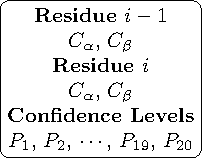
\includegraphics[width=\textwidth]{tile_fig}
	\end{center}
	\end{minipage}
\end{frame}

\begin{frame}
	\frametitle{Confidence Level Calculation}
	\begin{minipage}{0.45\textwidth}
		\begin{block}{Machine Learning}
			
		\end{block}
	\end{minipage}
	\begin{minipage}{0.45\textwidth}
	\begin{center}
		\huge\textbf{Tile}\\
		\vspace {12pt}
		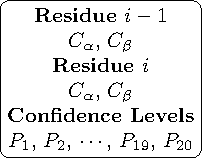
\includegraphics[width=\textwidth]{tile_fig}
	\end{center}
	\end{minipage}
\end{frame}

\begin{frame}
	\frametitle{Missing Data}
	\begin{minipage}{0.45\textwidth}
		\begin{block}{Blank Tile Creation}
			\begin{itemize}
				\item Compare length of protein sequence to NMR Data set
				\item Blank tiles are created to make up the gap
			\end{itemize}
		\end{block}
		\begin{block}{Proline}
			\begin{itemize}
				\item Lacks H-N spin system
				\item Does not produce $C_{\alpha}$, $C_{\beta}$ values
				\item Protein sequence is examined
				\item Special flags are set 
			\end{itemize}
		\end{block}
	\end{minipage}
	\begin{minipage}{0.45\textwidth}
	\begin{center}
		\huge\textbf{Blank Tile}\\
		\vspace {12pt}
		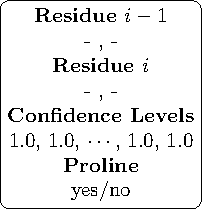
\includegraphics[width=\textwidth]{tile_fig_blank}
	\end{center}
	\end{minipage}
\end{frame}

\subsection{The Search} 
\begin{frame}
	\frametitle{Harvard University Conference}
	\begin{itemize}
		\item 1898
		\item Say some things
	\end{itemize}
\end{frame}

\section{Results}
\begin{frame}
	\frametitle{Machine Learning Algorithms}
	\resizebox{!}{0.6\textwidth}{% GNUPLOT: LaTeX picture with Postscript
\begingroup
  \makeatletter
  \providecommand\color[2][]{%
    \GenericError{(gnuplot) \space\space\space\@spaces}{%
      Package color not loaded in conjunction with
      terminal option `colourtext'%
    }{See the gnuplot documentation for explanation.%
    }{Either use 'blacktext' in gnuplot or load the package
      color.sty in LaTeX.}%
    \renewcommand\color[2][]{}%
  }%
  \providecommand\includegraphics[2][]{%
    \GenericError{(gnuplot) \space\space\space\@spaces}{%
      Package graphicx or graphics not loaded%
    }{See the gnuplot documentation for explanation.%
    }{The gnuplot epslatex terminal needs graphicx.sty or graphics.sty.}%
    \renewcommand\includegraphics[2][]{}%
  }%
  \providecommand\rotatebox[2]{#2}%
  \@ifundefined{ifGPcolor}{%
    \newif\ifGPcolor
    \GPcolortrue
  }{}%
  \@ifundefined{ifGPblacktext}{%
    \newif\ifGPblacktext
    \GPblacktexttrue
  }{}%
  % define a \g@addto@macro without @ in the name:
  \let\gplgaddtomacro\g@addto@macro
  % define empty templates for all commands taking text:
  \gdef\gplbacktext{}%
  \gdef\gplfronttext{}%
  \makeatother
  \ifGPblacktext
    % no textcolor at all
    \def\colorrgb#1{}%
    \def\colorgray#1{}%
  \else
    % gray or color?
    \ifGPcolor
      \def\colorrgb#1{\color[rgb]{#1}}%
      \def\colorgray#1{\color[gray]{#1}}%
      \expandafter\def\csname LTw\endcsname{\color{white}}%
      \expandafter\def\csname LTb\endcsname{\color{black}}%
      \expandafter\def\csname LTa\endcsname{\color{black}}%
      \expandafter\def\csname LT0\endcsname{\color[rgb]{1,0,0}}%
      \expandafter\def\csname LT1\endcsname{\color[rgb]{0,1,0}}%
      \expandafter\def\csname LT2\endcsname{\color[rgb]{0,0,1}}%
      \expandafter\def\csname LT3\endcsname{\color[rgb]{1,0,1}}%
      \expandafter\def\csname LT4\endcsname{\color[rgb]{0,1,1}}%
      \expandafter\def\csname LT5\endcsname{\color[rgb]{1,1,0}}%
      \expandafter\def\csname LT6\endcsname{\color[rgb]{0,0,0}}%
      \expandafter\def\csname LT7\endcsname{\color[rgb]{1,0.3,0}}%
      \expandafter\def\csname LT8\endcsname{\color[rgb]{0.5,0.5,0.5}}%
    \else
      % gray
      \def\colorrgb#1{\color{black}}%
      \def\colorgray#1{\color[gray]{#1}}%
      \expandafter\def\csname LTw\endcsname{\color{white}}%
      \expandafter\def\csname LTb\endcsname{\color{black}}%
      \expandafter\def\csname LTa\endcsname{\color{black}}%
      \expandafter\def\csname LT0\endcsname{\color{black}}%
      \expandafter\def\csname LT1\endcsname{\color{black}}%
      \expandafter\def\csname LT2\endcsname{\color{black}}%
      \expandafter\def\csname LT3\endcsname{\color{black}}%
      \expandafter\def\csname LT4\endcsname{\color{black}}%
      \expandafter\def\csname LT5\endcsname{\color{black}}%
      \expandafter\def\csname LT6\endcsname{\color{black}}%
      \expandafter\def\csname LT7\endcsname{\color{black}}%
      \expandafter\def\csname LT8\endcsname{\color{black}}%
    \fi
  \fi
  \setlength{\unitlength}{0.0500bp}%
  \begin{picture}(7200.00,5040.00)%
    \gplgaddtomacro\gplbacktext{%
      \csname LTb\endcsname%
      \put(814,1364){\makebox(0,0)[r]{\strut{}$10^0$}}%
      \csname LTb\endcsname%
      \put(814,1851){\makebox(0,0)[r]{\strut{}$10^1$}}%
      \csname LTb\endcsname%
      \put(814,2339){\makebox(0,0)[r]{\strut{}$10^2$}}%
      \csname LTb\endcsname%
      \put(814,2826){\makebox(0,0)[r]{\strut{}$10^3$}}%
      \csname LTb\endcsname%
      \put(814,3313){\makebox(0,0)[r]{\strut{}$10^4$}}%
      \csname LTb\endcsname%
      \put(814,3800){\makebox(0,0)[r]{\strut{}$10^5$}}%
      \csname LTb\endcsname%
      \put(814,4288){\makebox(0,0)[r]{\strut{}$10^6$}}%
      \csname LTb\endcsname%
      \put(814,4775){\makebox(0,0)[r]{\strut{}$10^7$}}%
      \csname LTb\endcsname%
      \put(1796,1144){\makebox(0,0){\strut{} 10}}%
      \csname LTb\endcsname%
      \put(2741,1144){\makebox(0,0){\strut{} 20}}%
      \csname LTb\endcsname%
      \put(3686,1144){\makebox(0,0){\strut{} 30}}%
      \csname LTb\endcsname%
      \put(4630,1144){\makebox(0,0){\strut{} 40}}%
      \csname LTb\endcsname%
      \put(5575,1144){\makebox(0,0){\strut{} 50}}%
      \csname LTb\endcsname%
      \put(6520,1144){\makebox(0,0){\strut{} 60}}%
      \put(176,3069){\rotatebox{-270}{\makebox(0,0){\strut{}Nodes Generated}}}%
      \put(3874,814){\makebox(0,0){\strut{}Number of Amino Acids}}%
    }%
    \gplgaddtomacro\gplfronttext{%
      \csname LTb\endcsname%
      \put(3019,393){\makebox(0,0)[r]{\strut{}No Filter}}%
      \csname LTb\endcsname%
      \put(3019,173){\makebox(0,0)[r]{\strut{}DecisionTable}}%
      \csname LTb\endcsname%
      \put(5590,393){\makebox(0,0)[r]{\strut{}J4.8}}%
      \csname LTb\endcsname%
      \put(5590,173){\makebox(0,0)[r]{\strut{}LMT}}%
    }%
    \gplbacktext
    \put(0,0){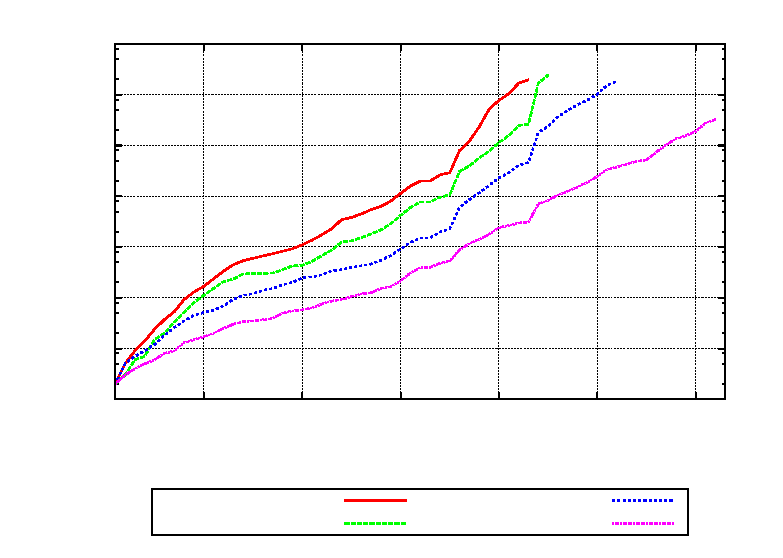
\includegraphics{ProFix_full}}%
    \gplfronttext
  \end{picture}%
\endgroup
}
\end{frame}

\begin{frame}
	\frametitle{Proline Checking}
	\resizebox{!}{0.6\textwidth}{% GNUPLOT: LaTeX picture with Postscript
\begingroup
  \makeatletter
  \providecommand\color[2][]{%
    \GenericError{(gnuplot) \space\space\space\@spaces}{%
      Package color not loaded in conjunction with
      terminal option `colourtext'%
    }{See the gnuplot documentation for explanation.%
    }{Either use 'blacktext' in gnuplot or load the package
      color.sty in LaTeX.}%
    \renewcommand\color[2][]{}%
  }%
  \providecommand\includegraphics[2][]{%
    \GenericError{(gnuplot) \space\space\space\@spaces}{%
      Package graphicx or graphics not loaded%
    }{See the gnuplot documentation for explanation.%
    }{The gnuplot epslatex terminal needs graphicx.sty or graphics.sty.}%
    \renewcommand\includegraphics[2][]{}%
  }%
  \providecommand\rotatebox[2]{#2}%
  \@ifundefined{ifGPcolor}{%
    \newif\ifGPcolor
    \GPcolortrue
  }{}%
  \@ifundefined{ifGPblacktext}{%
    \newif\ifGPblacktext
    \GPblacktexttrue
  }{}%
  % define a \g@addto@macro without @ in the name:
  \let\gplgaddtomacro\g@addto@macro
  % define empty templates for all commands taking text:
  \gdef\gplbacktext{}%
  \gdef\gplfronttext{}%
  \makeatother
  \ifGPblacktext
    % no textcolor at all
    \def\colorrgb#1{}%
    \def\colorgray#1{}%
  \else
    % gray or color?
    \ifGPcolor
      \def\colorrgb#1{\color[rgb]{#1}}%
      \def\colorgray#1{\color[gray]{#1}}%
      \expandafter\def\csname LTw\endcsname{\color{white}}%
      \expandafter\def\csname LTb\endcsname{\color{black}}%
      \expandafter\def\csname LTa\endcsname{\color{black}}%
      \expandafter\def\csname LT0\endcsname{\color[rgb]{1,0,0}}%
      \expandafter\def\csname LT1\endcsname{\color[rgb]{0,1,0}}%
      \expandafter\def\csname LT2\endcsname{\color[rgb]{0,0,1}}%
      \expandafter\def\csname LT3\endcsname{\color[rgb]{1,0,1}}%
      \expandafter\def\csname LT4\endcsname{\color[rgb]{0,1,1}}%
      \expandafter\def\csname LT5\endcsname{\color[rgb]{1,1,0}}%
      \expandafter\def\csname LT6\endcsname{\color[rgb]{0,0,0}}%
      \expandafter\def\csname LT7\endcsname{\color[rgb]{1,0.3,0}}%
      \expandafter\def\csname LT8\endcsname{\color[rgb]{0.5,0.5,0.5}}%
    \else
      % gray
      \def\colorrgb#1{\color{black}}%
      \def\colorgray#1{\color[gray]{#1}}%
      \expandafter\def\csname LTw\endcsname{\color{white}}%
      \expandafter\def\csname LTb\endcsname{\color{black}}%
      \expandafter\def\csname LTa\endcsname{\color{black}}%
      \expandafter\def\csname LT0\endcsname{\color{black}}%
      \expandafter\def\csname LT1\endcsname{\color{black}}%
      \expandafter\def\csname LT2\endcsname{\color{black}}%
      \expandafter\def\csname LT3\endcsname{\color{black}}%
      \expandafter\def\csname LT4\endcsname{\color{black}}%
      \expandafter\def\csname LT5\endcsname{\color{black}}%
      \expandafter\def\csname LT6\endcsname{\color{black}}%
      \expandafter\def\csname LT7\endcsname{\color{black}}%
      \expandafter\def\csname LT8\endcsname{\color{black}}%
    \fi
  \fi
  \setlength{\unitlength}{0.0500bp}%
  \begin{picture}(7200.00,5040.00)%
    \gplgaddtomacro\gplbacktext{%
      \csname LTb\endcsname%
      \put(814,1804){\makebox(0,0)[r]{\strut{}$10^0$}}%
      \csname LTb\endcsname%
      \put(814,2228){\makebox(0,0)[r]{\strut{}$10^1$}}%
      \csname LTb\endcsname%
      \put(814,2653){\makebox(0,0)[r]{\strut{}$10^2$}}%
      \csname LTb\endcsname%
      \put(814,3077){\makebox(0,0)[r]{\strut{}$10^3$}}%
      \csname LTb\endcsname%
      \put(814,3502){\makebox(0,0)[r]{\strut{}$10^4$}}%
      \csname LTb\endcsname%
      \put(814,3926){\makebox(0,0)[r]{\strut{}$10^5$}}%
      \csname LTb\endcsname%
      \put(814,4351){\makebox(0,0)[r]{\strut{}$10^6$}}%
      \csname LTb\endcsname%
      \put(814,4775){\makebox(0,0)[r]{\strut{}$10^7$}}%
      \csname LTb\endcsname%
      \put(1796,1584){\makebox(0,0){\strut{} 10}}%
      \csname LTb\endcsname%
      \put(2741,1584){\makebox(0,0){\strut{} 20}}%
      \csname LTb\endcsname%
      \put(3686,1584){\makebox(0,0){\strut{} 30}}%
      \csname LTb\endcsname%
      \put(4630,1584){\makebox(0,0){\strut{} 40}}%
      \csname LTb\endcsname%
      \put(5575,1584){\makebox(0,0){\strut{} 50}}%
      \csname LTb\endcsname%
      \put(6520,1584){\makebox(0,0){\strut{} 60}}%
      \put(176,3289){\rotatebox{-270}{\makebox(0,0){\strut{}Nodes Generated}}}%
      \put(3874,1254){\makebox(0,0){\strut{}Number of Amino Acids}}%
    }%
    \gplgaddtomacro\gplfronttext{%
      \csname LTb\endcsname%
      \put(4965,833){\makebox(0,0)[r]{\strut{}No Filter}}%
      \csname LTb\endcsname%
      \put(4965,613){\makebox(0,0)[r]{\strut{}Proline Check No Filter}}%
      \csname LTb\endcsname%
      \put(4965,393){\makebox(0,0)[r]{\strut{}LMT}}%
      \csname LTb\endcsname%
      \put(4965,173){\makebox(0,0)[r]{\strut{}Proline Check LMT}}%
    }%
    \gplbacktext
    \put(0,0){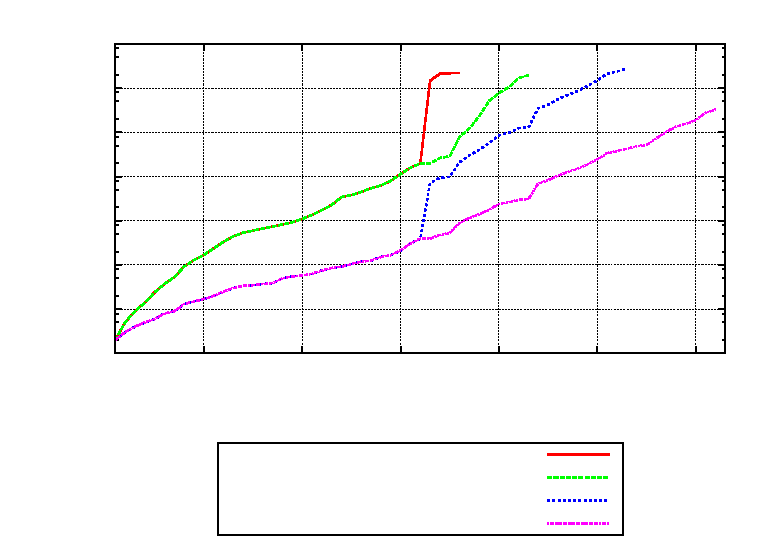
\includegraphics{pro_compare}}%
    \gplfronttext
  \end{picture}%
\endgroup
}
\end{frame}

\section{Outlook}
\begin{frame}
	\frametitle{Future Research}
	\begin{block}{Extend the Proline checking to other amino acids}
	\end{block}

	\begin{block}{Include a hysteric for assignment cost prediction}
	\end{block}

	\begin{block}{Assign subsets and combine to generate full assignments}
	\end{block}
\end{frame}

\section{}
\begin{frame}
	\frametitle{Thank You} 
	\begin{center}
		
	\end{center}
\end{frame}

\end{document}